\documentclass{homework}
% \usepackage{graphicx} % Required for inserting images
\usepackage{amsmath}
\usepackage{gensymb}
\usepackage{subfig}
\usepackage{float}

\class{ECEN 5738}
\title{Homework 6}
\author{Sean Jennings}
\date{April 22, 2024}

\newcommand{\K}{\mathcal{K}}
\renewcommand{\L}{\mathcal{L}}

\begin{document}
\maketitle

\section{Problem 1}
The impulse response $g$ relates the input $u$ to the output $y$
as follows
\begin{equation}
    y(t) = \int_{0}^{t} g(t - \tau) u(\tau) d\tau.
    \label{eq:y-impulse}
\end{equation}

Suppose $\norm{u}_{\L_1}$ is finite. Then,
\begin{align*}
    \norm{g}_{\L_1} \norm{u}_{\L_1} &= 
        \biggl(\int_{0}^{\infty} |g(s)| ds \biggr)
        \biggl(\int_{0}^{\infty} |u(\tau)| d\tau \biggr) \\
        &= \int_{0}^{\infty} \int_{0}^{\infty}
            |g(s)||u(\tau)| ds d\tau \\
        &= \int_{0}^{\infty} \int_{\tau}^{\infty}
            |g(t - \tau)||u(\tau)| dt d\tau
\end{align*}
using the substitution $s = t - \tau$.

This computation shows that the resulting double integral
converges absolutely. Therefore, we can exchange the order of 
integration:
\begin{equation*}
    \norm{g}_{\L_1} \norm{u}_{\L_1} = 
        \int_{0}^{\infty} \int_{0}^{t}
            |g(t - \tau)||u(\tau)| d\tau dt
\end{equation*}

From (\ref{eq:y-impulse}), we have
\begin{align*}
    \norm{y}_{\L_1} &= \int_{0}^{\infty}
        \biggl|\int_{0}^{t} g(t - \tau) u(\tau) d\tau \biggr|
        dt \\
        &\leq \int_{0}^{\infty}
            \int_{0}^{t} |g(t - \tau)| |u(\tau)| d\tau dt \\
        &= \norm{g}_{\L_1} \norm{u}_{\L_1}
\end{align*}
Thus, the system is finite gain stable with gain $\norm{g}_{\L_1}$.



\section{Problem 2}
A system is input-to-output stable if:
\begin{enumerate}
    \item it is ISS,
    \item The output $y = h(x, u)$ is bounded by:
        \begin{equation*}
            h(x, u) \leq \alpha_1 (\norm{x}) + \alpha_2 (\norm{u}) + \eta
        \end{equation*}
        where $\alpha_1$ and $\alpha_2$ are class-$\K$ functions
        and $\eta < \infty$ is a constant.
\end{enumerate}
Taking $\alpha_1 = \alpha_2 = (\cdot)^2$ and $\eta=0$, we see that
condition 2 holds with equality, so it remains to prove the system is
ISS.

Try the Lyapunov candidate $V(x) = 1/2 x^2$. The derivative is:
\begin{align*}
    \dot{V} = x \dot{x} &= x(-4x-x^3 + x^2 u) \\
        &= x^2 ( -4 -x^2 + xu) \\
        &\leq x^2( -4 -x^2 + 1/2x^2 + 1/2u^2) \\
        &= x^2 (1/2 u^2 - 1/2x^2 - 4)
\end{align*}
so whenever $\norm{x} \geq \norm{u}$, we have
\begin{equation*}
    1/2 u^2 - 1/2 x^2 \leq 0
\end{equation*}
and thus
\begin{equation*}
     1/2 u^2 - 1/2 x^2 -4 \leq -4 < 0
\end{equation*}
Thus, $\dot{V}(t) < 0$ whenever $\norm{x} \geq \norm{u}$,
the system is ISS, and consequently input-output stable.

\section{Problem 3}
We show the system is finite-gain $\mathcal{L}_2$ stable by
seperating the system into an equivalent interconnection of twothe nonlinear elements
subsystems: $H_1$ containing the linear elements, and $H_2$ contain
the nonlinear saturation function:

\begin{align*}
    \begin{array}{ll}
    H_1: \R \to \R  &\qquad                 H_2: \R \to \R \\
        \dot{x_1} = -x_1 + ax_2 &\qquad     y_2 = \frac{1}{2} \text{sat} (e_2) \\
        \dot{x_2} = bx_1 + cx_2 + e_1 \\ 
        y_1 = x_1 \\
    \end{array}
\end{align*}

\begin{center}
    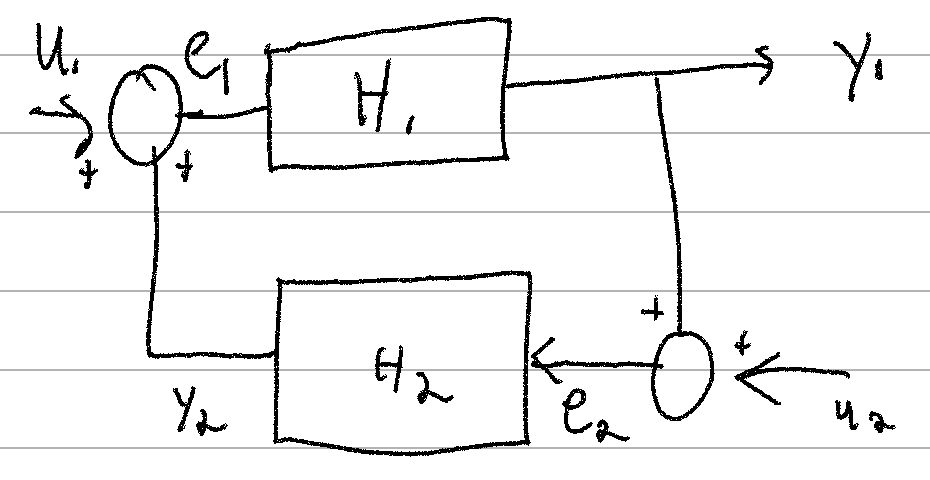
\includegraphics[width=0.8\linewidth]{Images/interconnect.png}
    \captionof{figure}{Separated interconection}
\end{center}

The following computation shows that the second
subsystem is finite gain $\mathcal{L}_2$ stable with
gain $\gamma_2 = 1/4$.

\begin{align*}
    \norm{y_2}_{\L 2} &= \int_{0}^{\infty} y_x^2(t) dt \\
        &= \int_{0}^{\infty} [\frac{1}{2} \text{sat}(e_2)]^2 dt \\
        &= 1/4 \int_{0}^{\infty} \text{sat}(e_2(t))^2 dt \\
        &\leq 1/4 \int_{0}^{\infty} e_2(t)^2 dt \\
        &= 1/4 \norm{e_2}_{\L 2}
\end{align*}

Since $H_2$ is linear, the gain can be found exactly, by
\begin{equation*}
    \gamma_1 = \sup_{\omega \in \R} G(j\omega)
\end{equation*}
where $G$ is the transfer function given by:
\begin{equation*}
    G(s) = C(sI - A)^{-1} B
\end{equation*}
and $A$, $B$ and $C$ are given by
\begin{equation*}
    A = \mat{-1 & a \\ b & c} \qquad B = \mat{0 \\ 1}
        \qquad C = \mat{1 & 0}
\end{equation*}

Let $D(s)$ be the characteristic polynomial of $A$:
\begin{equation*}
    D(s) = \det(sI - A) = s^2 + (c - 1) s - c - ab
\end{equation*}
Then,  we have 
\begin{equation*}
    (sI - A)^{-1} = \frac{1}{D(s)} \mat{
        s-c & a \\
        b & s+1
    }
\end{equation*}
and
\begin{equation*}
    G(s) = \frac{a}{D(s)} = \frac{a}{s^2 - (c-1) s - c - ab}
\end{equation*}

Since the numerator of $G$ is constant, the maximum $G(j\omega)$
occurs when $|D(j\omega)|$ is at a minimum.
\begin{equation*}
    |D(j\omega)|^2 = (\omega^2 + c + ab)^2 + (\omega(c-1))^2
\end{equation*}
So $|D(j\omega)| \to +\infty$ as $\omega$ approaches positive or negative
infinity.

Taking the derivative, we have
\begin{equation}
    2 \frac{d D(j\omega)}{d\omega} |D(j\omega)| =
        \frac{d}{d\omega}(|D(j\omega)|^2) = 
        2\omega ( 2\omega^2 + 2c + 2ab + (c-1)^2).
    \label{eq:deriv}
\end{equation}
Since for $a = 1, b = 2, c = -5$,  we have
\begin{equation*}
    2\omega^2 + 2c + 2ab + (c-1)^2 = 2\omega^2 + 30 > 0,
\end{equation*}
for all $\omega$, and we see that the derivative is 0 only at $\omega = 0$ and $|D(j\omega)|$
takes its minimum at $\omega = 0$.

Thus,
\begin{equation*}
    \gamma_1 = \sup_{\omega \in \R} G(j\omega) = G(0) = a / (-c - ab)
        = 1/3
\end{equation*}
and
\begin{equation*}
    \gamma_1 \cdot \gamma_2 = 1/12 < 1
\end{equation*}
so the small gain theorem can be applied to show that the system
is $\L_2$ stable.


\section{Problem 4: Dissipativity}

The system
\begin{align*}
    \dot{x} = f(x, u) \qquad f(0, 0) = 0
    y = h(x, u) \qquad h(0, 0) = 0
\end{align*}
is said to be \underline{dissipative} with respect to 
storage function $s(u, y)$ if $\exists V: \R^n \to \R$
such that
\begin{enumerate}
    \item V is a positive semidefinite function
    \item For all $x \in \R^n, u \in \R^m$
    \begin{equation}
        \nabla V(x)^T f(x, u) \leq s(u, h(x, u))
        \label{eq:dissipative-prop}
    \end{equation}
        holds.
\end{enumerate}

\begin{letterenum}
\item Since the time-derivative of $V$ along trajectories of
    the system is given by
    \begin{equation*}
        \dot{V}(t) = \nabla V(x(t))^T f(x(t), u(t)),
    \end{equation*}

    dissipativity with respect to $s$ implies that
    \begin{equation}
        \dot{V}(t) \leq s(u(t), y(t))
        \label{eq:dissipative-traj}
    \end{equation}
    along corresponding input/output trajectories $u$ and $y$.

    When the storage function is given by:
    \begin{equation}
        s(u, y) = \gamma \normtwo{u}^2 - \normtwo{y}^2
        \label{eq:l2-storage}
    \end{equation}
    rearranging terms in (\ref{eq:dissipative-traj}) yields
    \begin{equation*}
        \normtwo{y}^2 \leq \gamma \normtwo{u}^2 - \dot{V}
    \end{equation*}
    Integrating over the interval $[0, \tau]$, we have
    \begin{align*}
        \int_{0}^{\tau} \normtwo{y}^2 &= \gamma \int_{0}^{\tau} \normtwo{u(t)}^2 dt
                - \int_{0}^{\tau} \dot{V(t)}dt \\
            &= \gamma \int_{0}^{\tau} \normtwo{u(t)} dt - (V(\tau) - V(0)) \\
            &\leq \gamma \int_{0}^{\tau} \normtwo{u(t)} dt + V(0)
    \end{align*}
    since $V(t) \geq 0$.

    In the limit $\tau \to \infty$, we have
    \begin{equation*}
        \norm{y}_{\L 2} \leq \gamma \norm{u}_{\L 2} + V(0)
    \end{equation*}
    so the system is finite gain input-output $\L$-2 stable
    with gain $\gamma$.

\item For Lyapunov stability, we need a positive definite
$V$ which is negative semidefinite along trajectories which 
start in a certain region.

The system being dissipative with respect to the storage function
$s(u, y) = -\normtwo{y}^2$ implies that such a $V$ exists. For
by condition 1) of dissipativity, $V$ is positive definite and 
by condition 2), we have (when $u := 0$)
\begin{equation*}
    \dot{V} = \nabla V(x)^T f(x, 0) \leq -\normtwo{y}^2 \leq 0.
\end{equation*}

Any storage function $s(u, y)$ which has $s(0, y) \leq 0$ will
suffice to show Lyapunov stability for the control $u:=0$. One 
(set of) example(s) is the class of storage functions
\begin{equation*}
    s(u, y) = - y^T Q y
\end{equation*}
where $Q$ is a positive semi-definite matrix. Alternatively,
dissipativity with respect to an even degree monomial
function of the norm of $y$ such as
\begin{equation*}
    s(u, y) = - \norm{y}^4
\end{equation*}
will imply Lyapunov stability.

\item Dissipativity w.r.t. the storage function
$s(u, y) = \normtwo{u}^2$ implies that there exists a function
$V$ such that
\begin{equation*}
    \dot{V}(t) \leq \normtwo{u}^2
\end{equation*}
along all trajectories of the system.

Integrating with respect to time over the interval $[0, \tau]$
yields
\begin{align*}
    V(x(\tau)) - V(x(0)) = \int_{0}^{\tau} \dot{V}(t) dt
        \leq \int_0^\tau \normtwo{u(t)}^2 dt  \leq \norm{u}_{\L_2}
\end{align*}
Therefore, dissipativity implies $\L_2$ reachability because
\begin{equation*}
    V(x(\tau)) \leq V(x(0)) + \norm{u}_{\L_2} \leq \alpha + \beta.
\end{equation*}




\end{letterenum}












\end{document}
